\chapter{The Project}

\section{Architecture}

\begin{figure}[h]
    \centering
    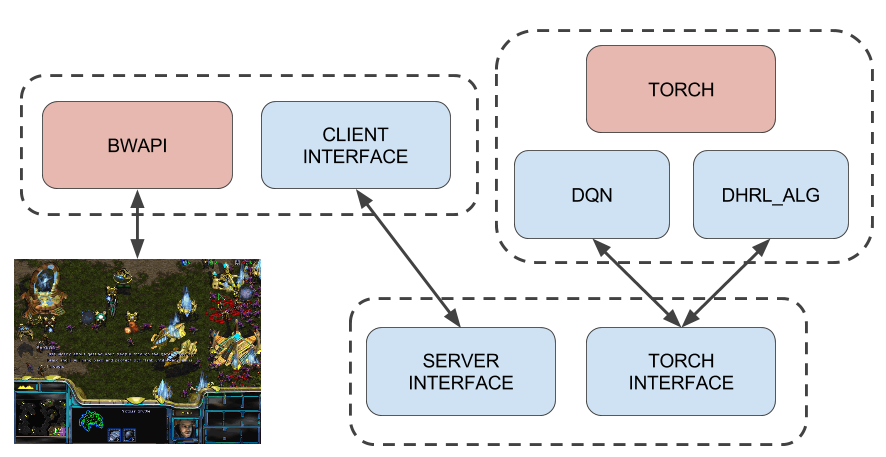
\includegraphics[width=\textwidth]{architecture}
    \caption{The project's current architecture}
    \label{fig:arch}
\end{figure}

Our entire architecture looks like the one in Figure \ref{fig:arch}: a C++
client initialises BWAPI and communicates through shared memory with a running
instance of StarCraft Brood War; the client is then linked to a server also
written in C++ running on a Linux machine through a blocking socket connection,
which initialises LuaJIT\cite{pall2008luajit}, Torch\cite{collobert2011torch},
the CUDA environment\cite{nvidia2008programming}, and then finally runs the AI.

The client not only manages the game and parses its information, but also takes
advantage of the standard Windows API to access the graphical output generated
by the game and extract it as a standard integer array, so that it can then sent
to the server and used as the input state for our algorithms together with the
game state. After several optimisation this operation doesn't take a significant
toll on the overall performances, but a text-based configuration system has also
been included to activate or deactivate features such as this one. The game
information is instead collected using BWAPI and then encoded in a Google
Protocol Buffer\cite{protobuf}, a standard serialisation object that encodes
arbitrary data structures into byte arrays and that is fast and that allows to
check for data presence and validity.

As we previously mentioned, BWAPI allows to do DLL injection and place the AI
binary code directly into the StarCraft process. This is the preferred method
used in both at SSCAIT and AIIDE (two StarCraft bots tournaments), but it
doesn't give a good amount of control on the game itself, and makes it therefore
difficult to prepare good experiment environments. Since those two methods are
exclusive, we decided to use the other client-server based interface. The idea
was to simulate most of the ALE interface to allow for easy interoperability
with DeepMind's DQN codebase and other codebases based on that particular one,
and the closest model was the one that was most decoupled from the game.

\section{C++ server to Torch: luajit interface}

After the game state and the image messages get passed through socket connection
to the linux server, those need to be passed to the lua process so that it can
own them and use them appropriately. To do so we wrapped the entire C++ server
interface in Lua objects by creating a dynamic library and loading it into Lua
using the LuaJIT interpreter.

LuaJIT is a Just-In-Time compiler for Lua, which allows to connect high
performance C and C++ code with the more high level Lua scripting language,
therefore simplifying the process of writing high-level interfaces while
maintaining the speed of faster but lower-level languages. There are a few ways
for this process to happen, but we essentially decided to directly load the
compiled binary with the C++ object definitions and declarations into the Lua
ecosystem via an LuaJIT internal declaration and linking system. The objects are
then wrapped with the Torch class interface[CITE HERE], which then can be used
completely without any worries in terms of memory management and threading (as
LuaJIT gives you a garbage collector for free as long as you set up the objects
in the proper way).

Translating the image was a slightly more difficult process, because the format
Windows uses to store bitmaps is largely unsupported one in the Linux ecosystem.
The conversion to the format used by Torch was optimised by noticing that the
colour channels are completely separate and that some pointer math was enough to
essentially allow us to use a threaded parallel loop and speed up the copying
process. We tried also acting on the stride information used by the Tensor
classes in Torch, but it made other operations very slow (all the ones that
actually modified the tensor itself), because the assumption of continuous data
array could not hold anymore for the rest of the libraries.

\section{Filtering the game state}

Because of its nature as an RTS, it's not easy to extract the totality of the
information that StarCraft produces within a game. In particular, it's not clear
in what ways a programmer should explore the state and which objects and
relations should be explicitly mapped out. For instance, it's possible to
retrieve spatial information about units and buildings, but collecting
information about all the technologies that each building can produce would mean
iterating through all the possible game objects, checking their existence and
creating a huge information tree, most of which is not necessarily useful to a
reinforcement learning system. To eliminate this problem we decide to limit our
experiments to a few unit classes and to retrieve only their positions and life
points, without caring about upgrades or other skills. The final set of unit
classes included only Terran and Zerg units, and were workers (of any kind),
soldiers (marines), healers (medics) and buildings. Because we were not sending
information about building usage, we also only needed to provide their position
and life points.

\section{Interfacing with DeepMind's DQN}

Once the interface was complete and most of the bugs were ironed out, we
proceeded to learn and adapt the code from DeepMind's Nature paper to work with
our project interface. Ultimately we made our interface look exactly like ALE's,
so that very few edits were needed to be made directly to their codebase.
However, a lot of code related to the different ATARI games was stripped and the
configuration layer was in general simplified.

Unsurprisingly, we discovered with a few preliminary tests that standard DQN was
simply not able to solve most of our maps. In particular, we individuated two
major issues to first address for basic deep Q-learning to successfully complete
even some basic part of the game.

\subsection{RTSs are inherently hierarchical}

As with all RTSs, the game forces players to focus on building solid overall
long-term game strategies and local short-term focused tactics completely in
parallel, often with the clear objective of making the player choose certain
trade-offs that will benefit long versus short term goals. As a strategy game, we
can therefore see that policies are structured and hierarchical, because certain
strategy might spawn certain tactics with parameters entirely dependent on the
``super-policy''. Additionally Starcraft is also hierarchical in its state and
value because of the existence of classes available only after certain inter
objectives have been reached, or even just because of the dependency on the
skill tree to develop both militarily and economically.

\subsection{Visual information are completely policy dependent}

As previously mentioned, with most of the roms used within ALE the visual data
contains the full state of the game. That is, assuming we have a good
understanding of the score function, the image given by ALE essentially gives us
all the information we need to model the most useful action at any given time
with reasonable results. In Starcraft the visual feedback purely represents the
state of the game at a specific point in the map - point usually chosen by the
player through keyboard or mouse actions - and unless the user puts time and
effort in dynamically exploring the map to update his world knowledge, they
can't get an idea of the general state of the game a part from looking at the
extremely compressed minimap (Figure \ref{fig:one_star}).

\begin{figure}[h]
    \centering
    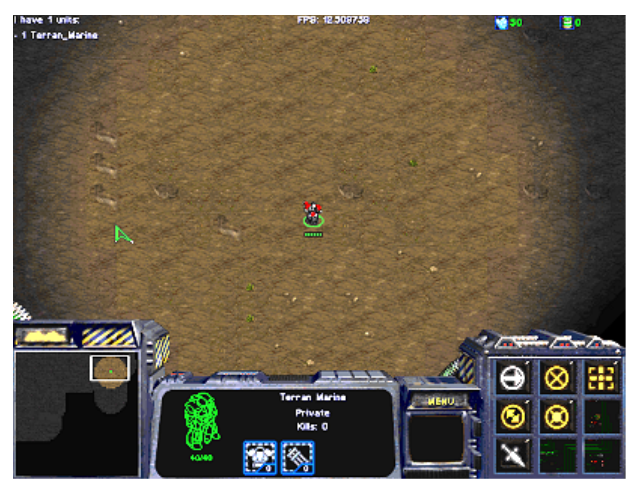
\includegraphics[width=\textwidth]{star_one}
    \caption{Standard StarCraft game screen that the player needs to interact
      with. The minimap is on the bottom-left; black areas are not yet
      discovered (and therefore not observable), grey areas have been discovered
      but are not fully observable anymore (topology of the map is known, unit
      or resources status is not) and light brown areas are observed areas with
      full observability in terms of game state (symbolical). The white
      rectangle signals the visible area at the current window position.}
    \label{fig:one_star}
\end{figure}

Additionally the minimap is also affected by the so-called Fog of War, a feature
in most RTS games that prevents players from observing the state of locally
explored but unobserved zones at a specific time. This means that to fully win
the game the player is forced to continuously explore the state of the game,
regardless of whether they have a more or less complete notion of the topology
of the map. In reality, Starcraft allows us to cheat and disable the Fog of War,
making exploration a one-shot process i.e. once the map is explored it’ll be
“observable” through the entirety of the match.

\begin{figure}[h]
    \centering
    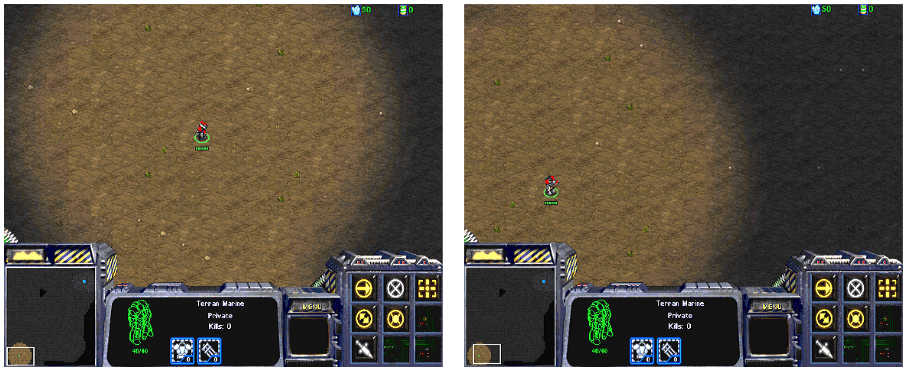
\includegraphics[width=\textwidth]{double_star}
    \caption{The variance in visual input between the two windows is as seen
      very high, because not only the relative position of the unit changes, but
      the entirety of the space changes significantly.}
    \label{fig:double_star}
\end{figure}

Starcraft’s visual feedback by itself (i.e. even without encoded features) is
therefore essentially non-Markovian in how it represents the state of the game.
Starcraft players are required to move the window to gain information, and the
image changes drastically depends on where the window is (Figure
\ref{fig:double_star}), so unless there is some form of memory to collect the
game state, we cannot only use the visual data as input. Our conjecture is that
creating an encoded representation of the entire state of game is by itself an
unsolved mixed deep learning (representation) and RL problem, as the variance in
the input is simply too large and it's entirely based on the learnt policy for
both unit actions and screen/environment actions.

\section{Tackling the hierarchical problem}

The issue itself is of policy learning. That is, theoretically we can imagine a
policy that maps all the possible states of the game, with the problem that it
would be clearly become too big even just considering two units and the smallest
map size (64 by 64 pixels). When we imagine games with hundreds of units, larger
maps and we add some unit data such as possible actions, life points, energy
points and further information the state quickly explodes and the problem
becomes hopelessly intractable. To try tackling this from a reinforcement
learning perspective we need to take advantage of the intrinsic hierarchy of
actions from a decision making point of view. We can then use techniques
originating from a the field called Hierarchical Reinforcement Learning.

The idea of splitting the learning process to tackle sub-problems and then
generalise over them has been a source of research for now a few decades.
Several techniques and methodologies have been invented over the years, some of
them trying to decompose the MDPs\cite{marthi2005concurrent} and act on the
decomposed value functions (MAXQ)\cite{dietterich2000hierarchical}, some of them
using generic gating mechanisms\cite{watkins1989learning}, some of them acting
directly in the policy and MDP space\cite{stolle2002learning}.

In our case, the simplest way to tackle StarCraft's policy problem is to
iteratively learn about useful sequences of actions, but to do this we need to
``guide'' the agent towards learning the correct primitives and we need to
tackle the simplest possible map, i.e. a map topologically flat in which within
its boundaries agents can move in all directions without constraints, where
there is only one type of enemy and controllable unit and where the only goal is
to maximise the time spent alive.

To learn the primitives we have created a series of random maps with close
boundaries where agents are forced to move mostly in one chosen direction.
Instead of specifically learning a policy, we instead learn the fitness value of
a specific action. Once we have done a few iterations and we know what are the
best actions, we combine them in several ways and we add those new combinations
to the set of possible actions. Doing this process until we stop creating useful
functions should allow us to discover useful primitives with different levels of
complexity.

Once we have learnt those primitives we can then test them with the
aforementioned flat map with additional units and then possibly use additional
models to control the global strategy of the units. The key idea is that we can
keep the same reward system and state representation by doing all this process
for each unit.

\newpage

\section{Final Semester Timeline}

The next steps to complete the project are included in the following table.

\begin{table}[h]
  \begin{center}
    \renewcommand\arraystretch{1.4}\arrayrulecolor{LightSteelBlue3}
    \captionsetup{singlelinecheck=false, font=blue, labelfont=sc, labelsep=quad}
    \caption{Timeline}\vskip -1.5ex
    \begin{tabular}{@{\,}r <{\hskip 2pt} !{\foo} >{\raggedright\arraybackslash}p{\textwidth}}
      \toprule
      \addlinespace[1.5ex]
      22nd January & Addition of infrastructure (no-model) for local primitive discovery. \\
      29th January & Implementation of learning model for local processes. \\
      5th February & Implementation of uniform state-representation and correct reward system. \\
      12th February & Evaluation and experiments on DQN. \\
      26th February & Evaluation and experiments on hierarchical processes. \\
      4th March & Beginning of report drafting process. \\
      11th March & Initial draft of project report. \\
      18th March & More work on project report. \\
      25th March & Final draft of project report. \\
      31st March & Submission of complete project report. \\
    \end{tabular}
  \end{center}
\label{tab:timeline}
\end{table}

